\documentclass[twoside]{book}

% Packages required by doxygen
\usepackage{calc}
\usepackage{doxygen}
\usepackage{graphicx}
\usepackage[utf8]{inputenc}
\usepackage{makeidx}
\usepackage{multicol}
\usepackage{multirow}
\usepackage{textcomp}
\usepackage[table]{xcolor}

% Font selection
\usepackage[T1]{fontenc}
\usepackage{mathptmx}
\usepackage[scaled=.90]{helvet}
\usepackage{courier}
\usepackage{amssymb}
\usepackage{sectsty}
\renewcommand{\familydefault}{\sfdefault}
\allsectionsfont{%
  \fontseries{bc}\selectfont%
  \color{darkgray}%
}
\renewcommand{\DoxyLabelFont}{%
  \fontseries{bc}\selectfont%
  \color{darkgray}%
}

% Page & text layout
\usepackage{geometry}
\geometry{%
  a4paper,%
  top=2.5cm,%
  bottom=2.5cm,%
  left=2.5cm,%
  right=2.5cm%
}
\tolerance=750
\hfuzz=15pt
\hbadness=750
\setlength{\emergencystretch}{15pt}
\setlength{\parindent}{0cm}
\setlength{\parskip}{0.2cm}
\makeatletter
\renewcommand{\paragraph}{%
  \@startsection{paragraph}{4}{0ex}{-1.0ex}{1.0ex}{%
    \normalfont\normalsize\bfseries\SS@parafont%
  }%
}
\renewcommand{\subparagraph}{%
  \@startsection{subparagraph}{5}{0ex}{-1.0ex}{1.0ex}{%
    \normalfont\normalsize\bfseries\SS@subparafont%
  }%
}
\makeatother

% Headers & footers
\usepackage{fancyhdr}
\pagestyle{fancyplain}
\fancyhead[LE]{\fancyplain{}{\bfseries\thepage}}
\fancyhead[CE]{\fancyplain{}{}}
\fancyhead[RE]{\fancyplain{}{\bfseries\leftmark}}
\fancyhead[LO]{\fancyplain{}{\bfseries\rightmark}}
\fancyhead[CO]{\fancyplain{}{}}
\fancyhead[RO]{\fancyplain{}{\bfseries\thepage}}
\fancyfoot[LE]{\fancyplain{}{}}
\fancyfoot[CE]{\fancyplain{}{}}
\fancyfoot[RE]{\fancyplain{}{\bfseries\scriptsize Generated on Tue Jun 21 2016 11\-:57\-:15 for My Controller R\-O\-S Package by Doxygen }}
\fancyfoot[LO]{\fancyplain{}{\bfseries\scriptsize Generated on Tue Jun 21 2016 11\-:57\-:15 for My Controller R\-O\-S Package by Doxygen }}
\fancyfoot[CO]{\fancyplain{}{}}
\fancyfoot[RO]{\fancyplain{}{}}
\renewcommand{\footrulewidth}{0.4pt}
\renewcommand{\chaptermark}[1]{%
  \markboth{#1}{}%
}
\renewcommand{\sectionmark}[1]{%
  \markright{\thesection\ #1}%
}

% Indices & bibliography
\usepackage{natbib}
\usepackage[titles]{tocloft}
\setcounter{tocdepth}{3}
\setcounter{secnumdepth}{5}
\makeindex

% Hyperlinks (required, but should be loaded last)
\usepackage{ifpdf}
\ifpdf
  \usepackage[pdftex,pagebackref=true]{hyperref}
\else
  \usepackage[ps2pdf,pagebackref=true]{hyperref}
\fi
\hypersetup{%
  colorlinks=true,%
  linkcolor=blue,%
  citecolor=blue,%
  unicode%
}

% Custom commands
\newcommand{\clearemptydoublepage}{%
  \newpage{\pagestyle{empty}\cleardoublepage}%
}


%===== C O N T E N T S =====

\begin{document}

% Titlepage & ToC
\hypersetup{pageanchor=false}
\pagenumbering{roman}
\begin{titlepage}
\vspace*{7cm}
\begin{center}%
{\Large My Controller R\-O\-S Package }\\
\vspace*{1cm}
{\large Generated by Doxygen 1.8.6}\\
\vspace*{0.5cm}
{\small Tue Jun 21 2016 11:57:15}\\
\end{center}
\end{titlepage}
\clearemptydoublepage
\tableofcontents
\clearemptydoublepage
\pagenumbering{arabic}
\hypersetup{pageanchor=true}

%--- Begin generated contents ---
\chapter{Namespace Index}
\section{Namespace List}
Here is a list of all documented namespaces with brief descriptions\-:\begin{DoxyCompactList}
\item\contentsline{section}{\hyperlink{namespacehiqp}{hiqp} }{\pageref{namespacehiqp}}{}
\end{DoxyCompactList}

\chapter{Hierarchical Index}
\section{Class Hierarchy}
This inheritance list is sorted roughly, but not completely, alphabetically\-:\begin{DoxyCompactList}
\item Joint\-Velocity\-Controller\begin{DoxyCompactList}
\item \contentsline{section}{hiqp\-:\-:Hi\-Q\-P\-\_\-\-Kinematic\-\_\-\-Controller}{\pageref{classhiqp_1_1HiQP__Kinematic__Controller}}{}
\end{DoxyCompactList}
\item \contentsline{section}{hiqp\-:\-:Task}{\pageref{classhiqp_1_1Task}}{}
\item \contentsline{section}{hiqp\-:\-:Task\-Manager}{\pageref{classhiqp_1_1TaskManager}}{}
\end{DoxyCompactList}

\chapter{Class Index}
\section{Class List}
Here are the classes, structs, unions and interfaces with brief descriptions\-:\begin{DoxyCompactList}
\item\contentsline{section}{\hyperlink{classhiqp_1_1HiQP__Kinematic__Controller}{hiqp\-::\-Hi\-Q\-P\-\_\-\-Kinematic\-\_\-\-Controller} \\*This is my awesome controller }{\pageref{classhiqp_1_1HiQP__Kinematic__Controller}}{}
\end{DoxyCompactList}

\chapter{File Index}
\section{File List}
Here is a list of all documented files with brief descriptions\-:\begin{DoxyCompactList}
\item\contentsline{section}{include/hiqp/\hyperlink{hiqp__kinematic__controller_8h}{hiqp\-\_\-kinematic\-\_\-controller.\-h} \\*Brief description of file }{\pageref{hiqp__kinematic__controller_8h}}{}
\item\contentsline{section}{include/hiqp/\hyperlink{hiqp__utils_8h}{hiqp\-\_\-utils.\-h} \\*Brief description of file }{\pageref{hiqp__utils_8h}}{}
\item\contentsline{section}{include/hiqp/\hyperlink{task_8h}{task.\-h} \\*Brief description of file }{\pageref{task_8h}}{}
\item\contentsline{section}{include/hiqp/\hyperlink{task__beh__fo_8h}{task\-\_\-beh\-\_\-fo.\-h} \\*Brief description of file }{\pageref{task__beh__fo_8h}}{}
\item\contentsline{section}{include/hiqp/\hyperlink{task__behaviour_8h}{task\-\_\-behaviour.\-h} \\*Brief description of file }{\pageref{task__behaviour_8h}}{}
\item\contentsline{section}{include/hiqp/\hyperlink{task__manager_8h}{task\-\_\-manager.\-h} \\*Brief description of file }{\pageref{task__manager_8h}}{}
\item\contentsline{section}{include/hiqp/\hyperlink{task__pop_8h}{task\-\_\-pop.\-h} \\*Brief description of file }{\pageref{task__pop_8h}}{}
\item\contentsline{section}{include/hiqp/\hyperlink{task__visualizer_8h}{task\-\_\-visualizer.\-h} \\*Brief description of file }{\pageref{task__visualizer_8h}}{}
\item\contentsline{section}{src/\hyperlink{hiqp__kinematic__controller_8cpp}{hiqp\-\_\-kinematic\-\_\-controller.\-cpp} \\*Brief description of file }{\pageref{hiqp__kinematic__controller_8cpp}}{}
\item\contentsline{section}{src/\hyperlink{hiqp__utils_8cpp}{hiqp\-\_\-utils.\-cpp} \\*Brief description of file }{\pageref{hiqp__utils_8cpp}}{}
\item\contentsline{section}{src/\hyperlink{task__beh__fo_8cpp}{task\-\_\-beh\-\_\-fo.\-cpp} \\*Brief description of file }{\pageref{task__beh__fo_8cpp}}{}
\item\contentsline{section}{src/\hyperlink{task__manager_8cpp}{task\-\_\-manager.\-cpp} \\*Brief description of file }{\pageref{task__manager_8cpp}}{}
\item\contentsline{section}{src/\hyperlink{task__pop_8cpp}{task\-\_\-pop.\-cpp} \\*Brief description of file }{\pageref{task__pop_8cpp}}{}
\item\contentsline{section}{src/\hyperlink{task__visualizer_8cpp}{task\-\_\-visualizer.\-cpp} \\*Brief description of file }{\pageref{task__visualizer_8cpp}}{}
\end{DoxyCompactList}

\chapter{Namespace Documentation}
\hypertarget{namespacemycontroller}{\section{mycontroller Namespace Reference}
\label{namespacemycontroller}\index{mycontroller@{mycontroller}}
}
\subsection*{Classes}
\begin{DoxyCompactItemize}
\item 
class \hyperlink{classmycontroller_1_1MyController}{My\-Controller}
\begin{DoxyCompactList}\small\item\em This is my awesome controller. \end{DoxyCompactList}\end{DoxyCompactItemize}


\subsection{Detailed Description}
namespace for mycontroller-\/related stuff 
\chapter{Class Documentation}
\hypertarget{classmycontroller_1_1MyController}{\section{mycontroller\-:\-:My\-Controller Class Reference}
\label{classmycontroller_1_1MyController}\index{mycontroller\-::\-My\-Controller@{mycontroller\-::\-My\-Controller}}
}


This is my awesome controller.  




{\ttfamily \#include $<$My\-Controller.\-h$>$}

Inheritance diagram for mycontroller\-:\-:My\-Controller\-:\begin{figure}[H]
\begin{center}
\leavevmode
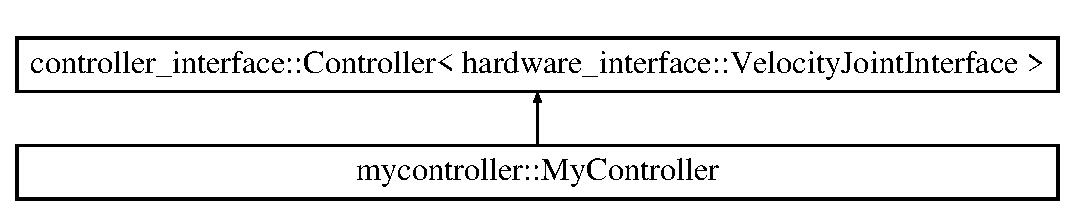
\includegraphics[height=2.000000cm]{classmycontroller_1_1MyController}
\end{center}
\end{figure}
\subsection*{Public Member Functions}
\begin{DoxyCompactItemize}
\item 
\hypertarget{classmycontroller_1_1MyController_a6f31f5a2318ff9e84accc3e3ce29e897}{\hyperlink{classmycontroller_1_1MyController_a6f31f5a2318ff9e84accc3e3ce29e897}{My\-Controller} ()}\label{classmycontroller_1_1MyController_a6f31f5a2318ff9e84accc3e3ce29e897}

\begin{DoxyCompactList}\small\item\em Constructor Constructs my awesome controller. \end{DoxyCompactList}\item 
\hypertarget{classmycontroller_1_1MyController_a30c609fe8c6f674a1d855bddd107f7f2}{\hyperlink{classmycontroller_1_1MyController_a30c609fe8c6f674a1d855bddd107f7f2}{$\sim$\-My\-Controller} () noexcept}\label{classmycontroller_1_1MyController_a30c609fe8c6f674a1d855bddd107f7f2}

\begin{DoxyCompactList}\small\item\em Destructor Destructs my awesome controller \-:(. \end{DoxyCompactList}\item 
bool \hyperlink{classmycontroller_1_1MyController_af9496597a461ffe70990e4a32a3d1cfd}{init} (hardware\-\_\-interface\-::\-Velocity\-Joint\-Interface $\ast$hw, ros\-::\-Node\-Handle \&controller\-\_\-nh)
\begin{DoxyCompactList}\small\item\em Called every time the controller is initialized by the ros\-::controller\-\_\-manager. \end{DoxyCompactList}\item 
bool \hyperlink{classmycontroller_1_1MyController_af16d743afe45456d6ad064d4a9e2860d}{starting} (const ros\-::\-Time \&time)
\begin{DoxyCompactList}\small\item\em Called every time the controller is started by the ros\-::controller\-\_\-manager. \end{DoxyCompactList}\item 
bool \hyperlink{classmycontroller_1_1MyController_a2839dfc2e9370ac8524b0f4e3bdd73c4}{update} (const ros\-::\-Time \&time, const ros\-::\-Duration \&period)
\begin{DoxyCompactList}\small\item\em Called every time the controller is updated by the ros\-::controller\-\_\-manager. \end{DoxyCompactList}\item 
bool \hyperlink{classmycontroller_1_1MyController_a2b7913b7eab96521a2ff14cda9afad3b}{stopping} (const ros\-::\-Time \&time)
\begin{DoxyCompactList}\small\item\em Called every time the controller is stopped by the ros\-::controller\-\_\-manager. \end{DoxyCompactList}\end{DoxyCompactItemize}


\subsection{Detailed Description}
This is my awesome controller. 

It's awesome! 

\subsection{Member Function Documentation}
\hypertarget{classmycontroller_1_1MyController_af9496597a461ffe70990e4a32a3d1cfd}{\index{mycontroller\-::\-My\-Controller@{mycontroller\-::\-My\-Controller}!init@{init}}
\index{init@{init}!mycontroller::MyController@{mycontroller\-::\-My\-Controller}}
\subsubsection[{init}]{\setlength{\rightskip}{0pt plus 5cm}bool mycontroller\-::\-My\-Controller\-::init (
\begin{DoxyParamCaption}
\item[{hardware\-\_\-interface\-::\-Velocity\-Joint\-Interface $\ast$}]{hw, }
\item[{ros\-::\-Node\-Handle \&}]{controller\-\_\-nh}
\end{DoxyParamCaption}
)}}\label{classmycontroller_1_1MyController_af9496597a461ffe70990e4a32a3d1cfd}


Called every time the controller is initialized by the ros\-::controller\-\_\-manager. 

Does some cool stuff!


\begin{DoxyParams}{Parameters}
{\em hw} & \-: a pointer to the hardware interface used by this controller \\
\hline
{\em controller\-\_\-nh} & \-: the node handle of this controller \\
\hline
\end{DoxyParams}
\begin{DoxyReturn}{Returns}
true if the initialization was successful 
\end{DoxyReturn}
\hypertarget{classmycontroller_1_1MyController_af16d743afe45456d6ad064d4a9e2860d}{\index{mycontroller\-::\-My\-Controller@{mycontroller\-::\-My\-Controller}!starting@{starting}}
\index{starting@{starting}!mycontroller::MyController@{mycontroller\-::\-My\-Controller}}
\subsubsection[{starting}]{\setlength{\rightskip}{0pt plus 5cm}bool mycontroller\-::\-My\-Controller\-::starting (
\begin{DoxyParamCaption}
\item[{const ros\-::\-Time \&}]{time}
\end{DoxyParamCaption}
)}}\label{classmycontroller_1_1MyController_af16d743afe45456d6ad064d4a9e2860d}


Called every time the controller is started by the ros\-::controller\-\_\-manager. 

Does some cool stuff!


\begin{DoxyParams}{Parameters}
{\em time} & \-: the current wall-\/time in R\-O\-S \\
\hline
\end{DoxyParams}
\begin{DoxyReturn}{Returns}
true if the starting was successful 
\end{DoxyReturn}
\hypertarget{classmycontroller_1_1MyController_a2b7913b7eab96521a2ff14cda9afad3b}{\index{mycontroller\-::\-My\-Controller@{mycontroller\-::\-My\-Controller}!stopping@{stopping}}
\index{stopping@{stopping}!mycontroller::MyController@{mycontroller\-::\-My\-Controller}}
\subsubsection[{stopping}]{\setlength{\rightskip}{0pt plus 5cm}bool mycontroller\-::\-My\-Controller\-::stopping (
\begin{DoxyParamCaption}
\item[{const ros\-::\-Time \&}]{time}
\end{DoxyParamCaption}
)}}\label{classmycontroller_1_1MyController_a2b7913b7eab96521a2ff14cda9afad3b}


Called every time the controller is stopped by the ros\-::controller\-\_\-manager. 

Does some cool stuff!


\begin{DoxyParams}{Parameters}
{\em time} & \-: the current wall-\/time in R\-O\-S \\
\hline
\end{DoxyParams}
\begin{DoxyReturn}{Returns}
true if the stopping was successful 
\end{DoxyReturn}
\hypertarget{classmycontroller_1_1MyController_a2839dfc2e9370ac8524b0f4e3bdd73c4}{\index{mycontroller\-::\-My\-Controller@{mycontroller\-::\-My\-Controller}!update@{update}}
\index{update@{update}!mycontroller::MyController@{mycontroller\-::\-My\-Controller}}
\subsubsection[{update}]{\setlength{\rightskip}{0pt plus 5cm}bool mycontroller\-::\-My\-Controller\-::update (
\begin{DoxyParamCaption}
\item[{const ros\-::\-Time \&}]{time, }
\item[{const ros\-::\-Duration \&}]{period}
\end{DoxyParamCaption}
)}}\label{classmycontroller_1_1MyController_a2839dfc2e9370ac8524b0f4e3bdd73c4}


Called every time the controller is updated by the ros\-::controller\-\_\-manager. 

Does some cool stuff!


\begin{DoxyParams}{Parameters}
{\em time} & \-: the current wall-\/time in R\-O\-S \\
\hline
{\em period} & \-: the time between the last update call and this, i.\-e. the sample time. \\
\hline
\end{DoxyParams}
\begin{DoxyReturn}{Returns}
true if the update was successful 
\end{DoxyReturn}


The documentation for this class was generated from the following file\-:\begin{DoxyCompactItemize}
\item 
mycontroller/include/\hyperlink{MyController_8h}{My\-Controller.\-h}\end{DoxyCompactItemize}

\chapter{File Documentation}
\hypertarget{MyController_8h}{\section{mycontroller/include/\-My\-Controller.h File Reference}
\label{MyController_8h}\index{mycontroller/include/\-My\-Controller.\-h@{mycontroller/include/\-My\-Controller.\-h}}
}


My\-Controller is my super-\/nice controller.  


{\ttfamily \#include $<$string$>$}\\*
{\ttfamily \#include $<$vector$>$}\\*
{\ttfamily \#include $<$boost/shared\-\_\-ptr.\-hpp$>$}\\*
{\ttfamily \#include $<$ros/ros.\-h$>$}\\*
{\ttfamily \#include $<$ros/node\-\_\-handle.\-h$>$}\\*
{\ttfamily \#include $<$controller\-\_\-interface/controller.\-h$>$}\\*
{\ttfamily \#include $<$hardware\-\_\-interface/joint\-\_\-command\-\_\-interface.\-h$>$}\\*
\subsection*{Classes}
\begin{DoxyCompactItemize}
\item 
class \hyperlink{classmycontroller_1_1MyController}{mycontroller\-::\-My\-Controller}
\begin{DoxyCompactList}\small\item\em This is my awesome controller. \end{DoxyCompactList}\end{DoxyCompactItemize}
\subsection*{Namespaces}
\begin{DoxyCompactItemize}
\item 
\hyperlink{namespacemycontroller}{mycontroller}
\end{DoxyCompactItemize}


\subsection{Detailed Description}
My\-Controller is my super-\/nice controller. \begin{DoxyAuthor}{Author}
Marcus A Johansson 
\end{DoxyAuthor}
\begin{DoxyVersion}{Version}
0.\-1 
\end{DoxyVersion}
\begin{DoxyDate}{Date}
2016-\/06-\/21 
\end{DoxyDate}

%--- End generated contents ---

% Index
\newpage
\phantomsection
\addcontentsline{toc}{chapter}{Index}
\printindex

\end{document}
